\documentclass[10pt,aspectratio=1610,professionalfont]{beamer}

%=========================
%        packages
%=========================
\usepackage[progressbar=frametitle]{beamerthememetropolis}
\usepackage{appendixnumberbeamer}
\usepackage{booktabs}
\usepackage{pgfplots}
\usepackage{amsmath}
\usepgfplotslibrary{dateplot}
\usepackage{xspace}
\usepackage[colorinlistoftodos]{todonotes}
\usepackage{caption}
\usepackage{subcaption}
\usepackage[many]{tcolorbox}
\usepackage{multicol}
\usepackage{etoolbox}
% get environments infobox, bluehighlight, redhighlight
\newenvironment{infobox}[1]{\begin{tcolorbox}[colback=mDarkTeal!10!white,
colframe=mDarkTeal,
                     title=\textsc{#1},  
                     center, 
                     valign=top, 
                     halign=left,
                     before skip=0.8cm, 
                     after skip=1.2cm,
                     center title, 
                     outer arc=0mm,
                     boxrule=0.2pt,
                     width=\textwidth]
}{}

\newenvironment{highlightbox}[2]{
	\begin{tcolorbox}[
		colback=#1!10!white,
		colframe=#1,  
		valign=center, 
        halign=left,
        before skip=0.3cm, 
        after skip=0.5cm,
        center title, 
        arc=0mm,
		boxrule=0.2pt,
        leftrule=3mm,
        width=#2\textwidth]
       \small
}{\normalsize\end{tcolorbox}}

\newenvironment{tagbox}{\begin{tcolorbox}[colback=mLightBrown!10!white,
colframe=mLightBrown,  size=fbox]
}{\end{tcolorbox}}




%=========================
%         colors
%=========================

\definecolor{mDarkGray}{HTML}{363d41}
\definecolor{mLightGray}{HTML}{d2dadd}
\definecolor{mRed}{HTML}{CC1C14}
\definecolor{mBlue}{HTML}{203c56}
\definecolor{mGreen}{HTML}{14cc33}
\definecolor{mPurple}{HTML}{882291}
\definecolor{mTeal}{HTML}{22917d}

%=========================
%       Title page
%=========================

\title{This is my medium length title}
\subtitle{Sometimes you need a subtitle which can even be longer}
\author{Alexander Franke}
\date{\today}
\institute{Universität Hamburg\\Fachbereich Physik}
%\titlegraphic{\hfill\includegraphics[height=1.5cm]{logo.pdf}}

%=========================
%          Fonts
%=========================
\usepackage[no-math]{fontspec}
\setmainfont[Ligatures=TeX]{AlegreyaSansSC-Regular.otf}
%\usepackage{gfsneohellenicot}
%\usepackage[default]{sourcesanspro}
\setsansfont{AlegreyaSans-Regular.otf}
%\usefonttheme[onlymath]{serif}
\usepackage{MnSymbol}
\usepackage[MnSymbol]{mathspec}
\setmathfont(Digits,Latin)[Lowercase=Regular,Uppercase=Regular]{AlegreyaSans-Regular.otf}
\setmathfont(Greek)[Lowercase=Regular,Uppercase=Regular,Scale=0.95]{AlegreyaSans-Regular.otf}
\AtBeginEnvironment{align}{\large}
\AtEndEnvironment{align}{\normalsize}
\usepackage{graphicx}
\renewcommand*\partial{\textsf{\reflectbox{6}}}
\setbeamertemplate{itemize item}{\large\guillemotright\normalsize}
\setbeamertemplate{itemize subitem}{\large\guilsinglright\normalsize}





%_________________________________________
%_________________________________________

\begin{document}
\maketitle

\begin{frame}{Outline}
 \setbeamertemplate{section in toc}[sections numbered]
  \tableofcontents
\end{frame}
%_______________________________________________________________________________
\section{Motivation}
\begin{frame}{MassQ Comsol Simulations}
\begin{figure}[!htb]
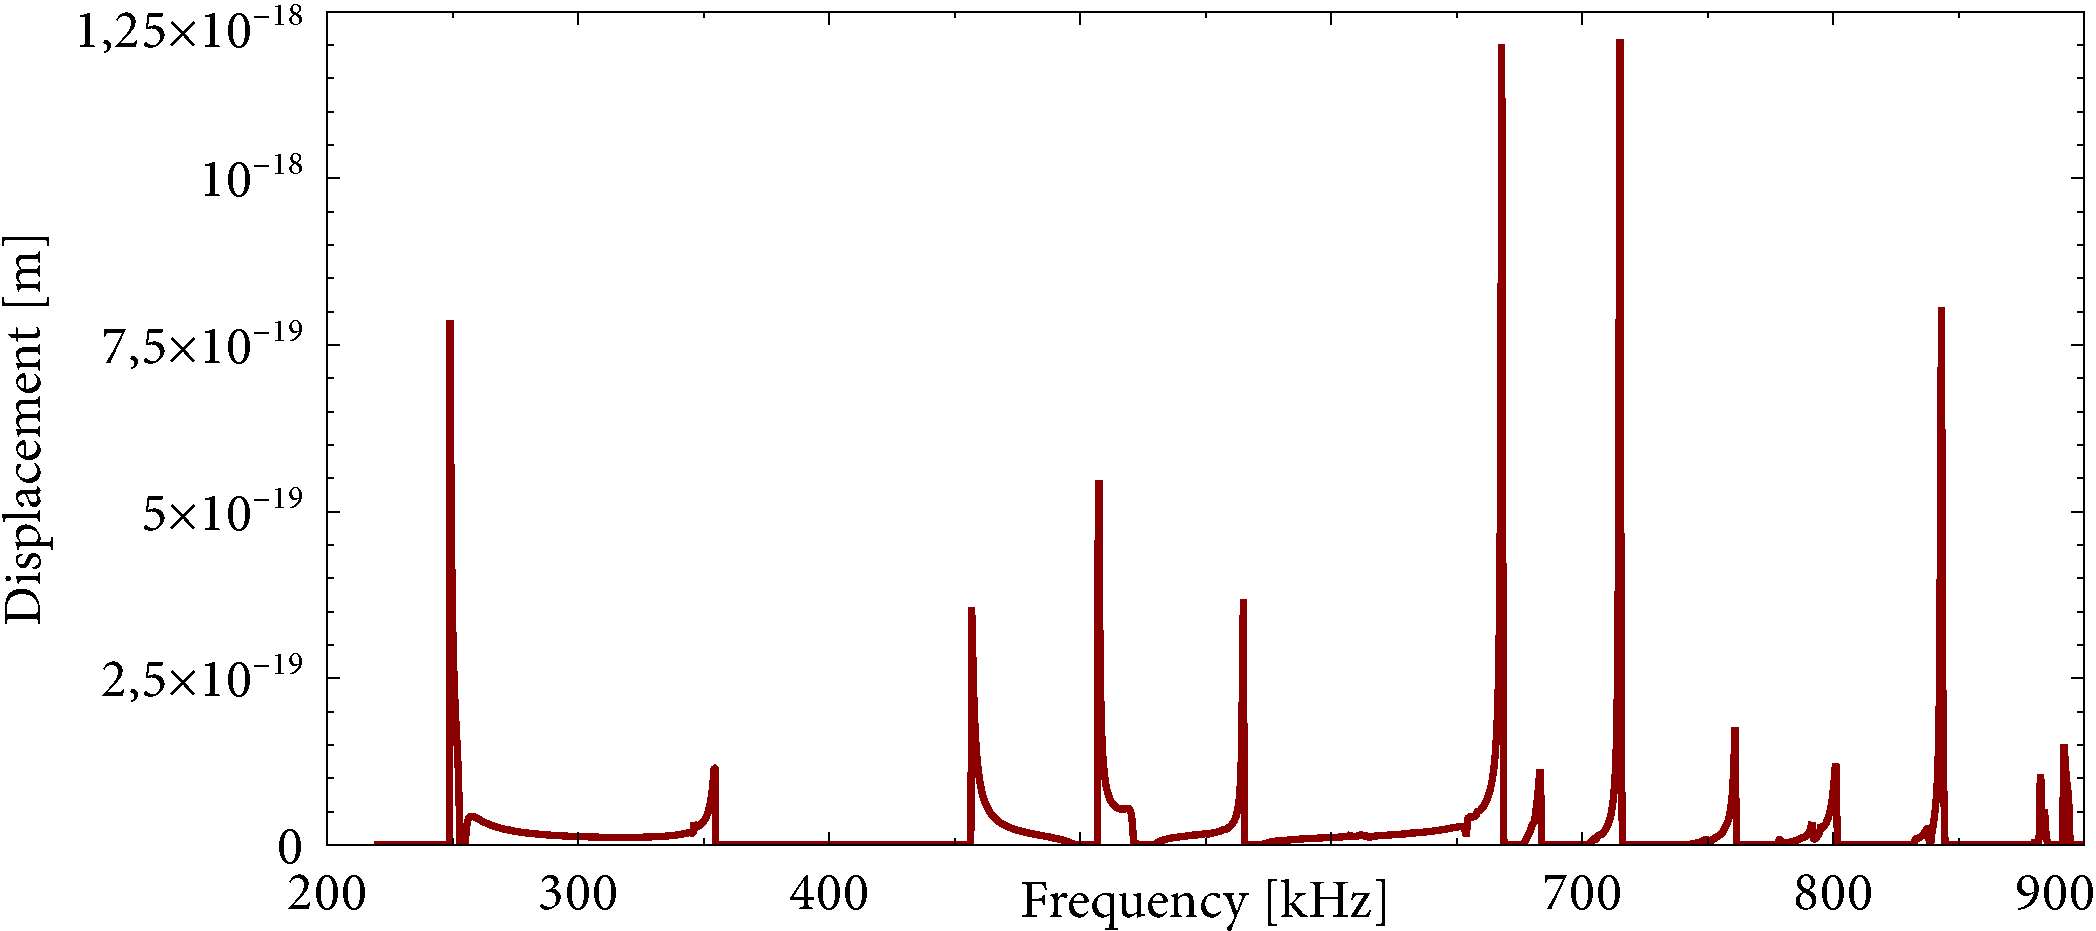
\includegraphics[width=0.9\textwidth]{testmass_response.pdf}
\caption{Round \alert{Testmass}. Harmonic body force: 0.01\,N. Gaussian beam width FWHM: $0.2\text{R}_\text{Testmass}$}
\end{figure}
\end{frame}

\begin{frame}{This week}

%\tcbox[size=fbox]{afs}
\begin{multicols}{2}
\begin{itemize}
\item Testmass Frequency response seen by a gaussian beam hitting one side in the middle with a 1/5 radius of the testmass radius
\begin{itemize}
\item subitem
\begin{itemize}
\item subsubitem
\end{itemize}
\end{itemize}

\item Testmass   Frequency response seen by a gaussian beam hitting one side in the middle with a 1/5 radius of the testmass  radius abx $abx$ and the \textmu m

\end{itemize}
\begin{align}
 \int_a^b \mu\pi x^2\;dx= \tfrac{1}{3} x^3 \Big|_a^b \circledR \\
  \mu \alpha \beta \gamma \delta \epsilon \phi \theta \vartheta \pi \chi \xi \Xi \\
  \frac{\partial}{\partial x} \left[ \sqrt[2]{\frac{e^{-i\omega t}}{4 \pi \epsilon_0}} \right]
\end{align}
\end{multicols}
\end{frame}
\section{boxes}

\begin{frame}{highlightbox test fi}
\alert{This is a example frame for different boxes}
	\begin{highlightbox}{mBlue}{.5}
			This is a mBlue highlight box
		\end{highlightbox}
		\begin{highlightbox}{mRed}{.5}
			This is a mRed highlight box
		\end{highlightbox}
		\begin{highlightbox}{mTeal}{.5}
			This is a mTeal highlight box
		\end{highlightbox}
		\begin{highlightbox}{mPurple}{.5}
			This is a mPurple highlight box
		\end{highlightbox}
\end{frame}
\begin{frame}{Zwei Spalten}
\begin{multicols}{2}
		Lorem ipsum dolor sit amet, consetetur sadipscing elitr, sed diam nonumy eirmod tempor invidunt ut labore et dolore magna aliquyam erat, sed diam voluptua. At vero eos et accusam et justo duo dolores et ea rebum. Stet clita kasd gubergren, no sea takimata sanctus est Lorem ipsum dolor sit amet.
		\begin{highlightbox}{mGreen}{.5}
			This is a green highlight box
		\end{highlightbox}
	\end{multicols}

\end{frame}
\end{document}
